% Drawing 69/04-9 -- folder 69, batch 04, archive page 61 (PDF page 62).
% Transcription: tableau, ligne $12^\circ$, première colonne : un petit dessin (la « demi-étoile ») --- cinq gros points alignés sur une horizontale, chacun relié à un sommet supérieur et à un sommet inférieur communs ; les deux premiers forment avec ces sommets un losange et sa diagonale, les trois autres sont joints par des arcs de plus en plus longs.
% Kind: two vertices joined to five aligned points (the half-star). Method 2 (schematic redraw from the facsimile). Status: ok.
% Notes: As on the page: five heavy points in a row, an upper vertex above the second point and a lower vertex below it, and from each of the five points one edge to the upper vertex and one to the lower vertex, all drawn between the same points (ten edges); the edges of the three right-hand points are slightly curved on the page (drawn as curves for the two outer ones). Left out: the cell borders of the table. The note of the transcription describes it as « un losange avec des arcs issus d'un sommet »: on the page the arcs join both vertices, upper and lower, to each of the five points. Redrawn 2026-11-12 (issue 128): to check again.
% Coordinates: 1 unit = 0.4 mm = 1/100 of the crop width (bbox in page fractions: [0.24, 0.578, 0.32, 0.61]).
% Redrawn by Claude (claude-fable-5-2), issue #128, 2026-11-12; not checked by a human; not compiled (no TeX in the session).
% Rights: reproduces part of the work -- behind RENDER_TRANSCRIPTS, never published by itself.
\documentclass[tikz,border=3pt]{standalone}
\usepackage{amsmath,amssymb}
\usetikzlibrary{patterns,arrows.meta}
\tikzset{pencil/.style={black!45}, struck/.style={black!35}, mpt/.style={circle,draw,inner sep=1.3pt}, pt/.style={circle,fill,inner sep=0.9pt}, opt/.style={circle,draw,fill=white,inner sep=1.1pt}}
\begin{document}
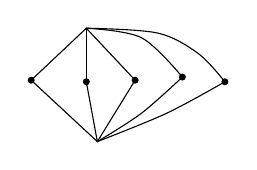
\begin{tikzpicture}[x=0.4mm,y=0.4mm,line cap=round,line join=round,font=\scriptsize]
\node[pt] at (5,-31.5) {};
\node[pt] at (22.5,-32) {};
\node[pt] at (38,-31.5) {};
\node[pt] at (53,-30.5) {};
\node[pt] at (66.5,-32) {};
\draw (22.5,-15) -- (5,-31.5);
\draw (5,-31.5) -- (26,-51);
\draw (22.5,-15) -- (22.5,-32);
\draw (22.5,-32) -- (26,-51);
\draw (22.5,-15) -- (38,-31.5);
\draw (38,-31.5) -- (26,-51);
\draw plot[smooth, tension=0.55] coordinates {(22.5,-15) (40,-18) (53,-30.5)};
\draw plot[smooth, tension=0.55] coordinates {(53,-30.5) (40,-42) (26,-51)};
\draw plot[smooth, tension=0.55] coordinates {(22.5,-15) (45,-16.5) (58,-23) (66.5,-32)};
\draw plot[smooth, tension=0.55] coordinates {(66.5,-32) (48,-42) (26,-51)};
\end{tikzpicture}
\end{document}
